\ifdefined\included
\else
\setcounter{chapter}{7} %% Numéro du chapitre précédent ;)
\dominitoc
\faketableofcontents
\fi

\chapter{Moving forward binary relations in the REG}
\minitoc

The contribution presented in this chapter is a preliminary work aiming to consider the limitations encountered by the contribution of the previous chapter. The presented method has been implemented but not tested with an integration of other components. This section deviates a little from the field of HRI to be more anchored in artificial intelligence. However, the ability to generate entity referencing in a more generic way is paramount for a robot to interact with humans. 

\section{Introduction}

Representing the whole complexity of the knowledge composing our world into a machine-readable language is a central issue in artificial intelligence. Coming from the Semantic Web, we saw that the use of an ontology through RDF-based languages succeeded in establishing itself in the field of artificial intelligence and therefore robotics. Although, what is often viewed as a limitation of ontology is its capability to only represent unary and binary relations. Binary relations such as \textit{"Sean Connery has the British nationality"} are described through the form of triples \textit{(sean\_connery, hasNationality, british)}. Unary relation such as \textit{"Sean Connery is an actor"} can them be transformed into binary relation through the addition of dedicated predicates \textit{(sean\_connery, isA, Actor)}. However, the description of more complex relations involving more than two entities is must more challenging using such representation.

Taking the example of Sean Connery\footnote{In the case you do not know who is Sean Connery feel free to take another actor that you like but you will have to adapt the entire example. Good luck.}, f we want to refer to him\footnote{Obviously we want to refer to him without his name since we consider a person having recognized himself in the previous note.}, we could state that he is the actor playing the role of James Bond. However, other actor played this role. We could also say that he is the actor playing in the film Gold finger but once again others do. We could finally explain that he is the actor playing the role of James Bond and playing in the film Gold Finger. However, limiting us to the use of binary relations modify the exact information. A more accurate description would be that he is the actor playing the role of James Bond in the film Gold Finger. Here we see the necessity of relations involving more than two entities. In our example, we need to link the three entities that are the actor "Sean Connery", the role "James Bond", and the film "Gold Finger". Together, they describe a performance. Without being explicitly linked all three theses information would not represent the performance. Moreover, without these links, we could give an explanation such as the actor playing the role of James Bond and playing in the film Rising Sun. Both information is true but does not make sense together.

%Even if no standard pattern has been approved by the W3C for n-ary relations, they can still be represented indirectly. In this section, we start by describing the usual way to represent n-ary relations \cite{giunti_representing_2019}, which we will call \textbf{Compound Relations} (CR) because of the composition of binary relations to represent them. Then, we present an algorithm to pre-process them with the objective to facilitate their use in the REG algorithm.

\section{Related work: A richer knowledge representation with n-ary relations}

\begin{figure}[ht!]
\centering
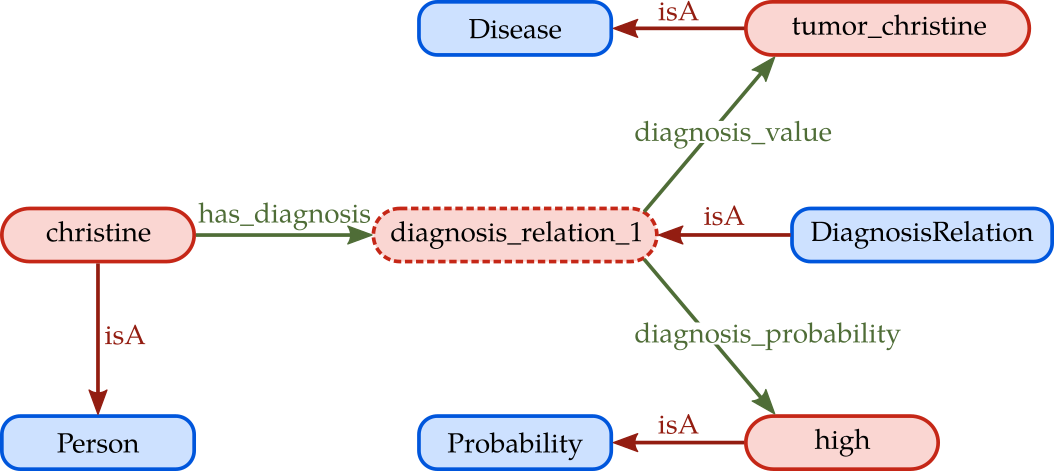
\includegraphics[scale=0.4]{figures/chapter7/w3c_p1.png}
\caption{\label{fig:chap7_w3c_p1} Ontological pattern 1 with subject proposed by the W3C Working Group.}
\end{figure}

\begin{figure}[ht!]
\centering
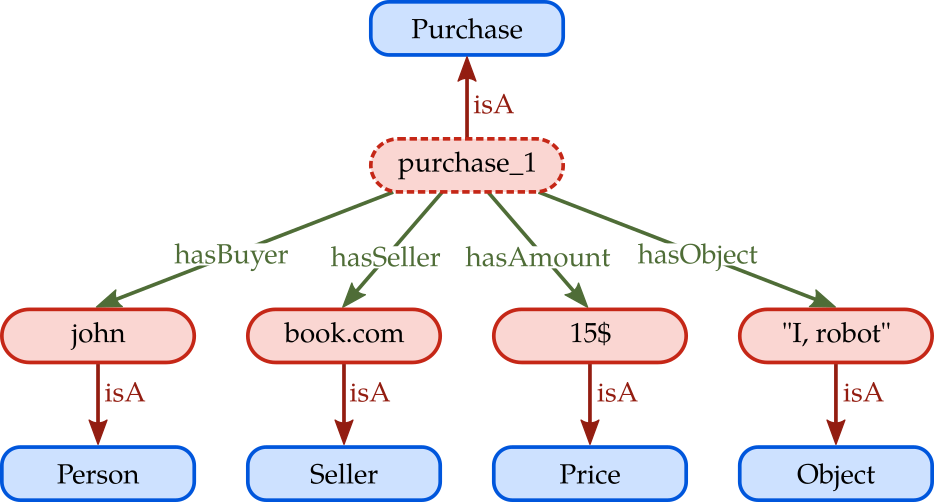
\includegraphics[scale=0.4]{figures/chapter7/w3c_p2.png}
\caption{\label{fig:chap7_w3c_p2} Ontological pattern 1 without subject proposed by the W3C Working Group.}
\end{figure}

\begin{figure}[ht!]
\centering
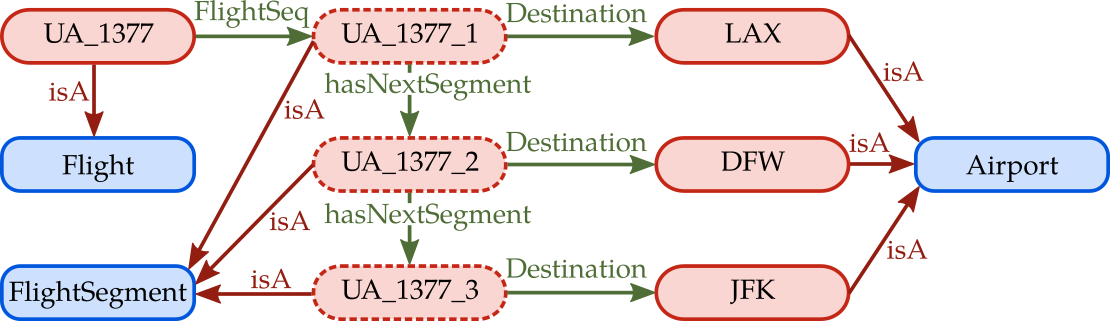
\includegraphics[scale=0.4]{figures/chapter7/w3c_p3.png}
\caption{\label{fig:chap7_w3c_p3} Ontological pattern 2 with subject proposed by the W3C Working Group.}
\end{figure}


\section{Through the use of coumpound relations}

\subsection{Defining a compound relation}

\subsection{A light way of representing the verbal link}

\subsection{A strategy to explore compund relations}

\subsubsection{A naive startegy to explore compound relations}

\subsubsection{A advanced strategy to explore compound relations}


\section{Generating Referring Expression wit compound relations}

\subsection{Determining a referring expression validity}

\subsection{Exploring the compound relations}

\subsection{From tree to radix tree}


\section{Results}

\subsection{The actor playing James Bond}

\subsection{The desciption of past activities as compound relations}